\section{Related Work Methodology Outtakes}
Marian suggests I aim for writing brief, one-paragraph summaries and apply the T tactic of the broad literature, the top bar of the T are the many and various papers on a topic, and I'm picking these ones that are most directly germane to my research which become the vertical bar of the T.\todo{I'm still currently more verbose than this :(} 

Marian also suggested I might end up with two or a maximum of 3 levels of Ts. The higher level would be on Software Quality Improvement. The lower level would be on mobile analytics.

\section{Introduction to the related work}
% Reinstate the following once I've completed the first complete draft of the following sections.
% starting with research into app stores and their effects on software development and engineering \ref{rw-app-stores-and-their-effects-on-software-development-and-engineering}...

\section{Software Development}
% For the purposes of this research there are at least two camps in research. The first camp is where the research comes from the field and is applied in the field of production, shipping software and the second camp seeks ways to improve the tools, techniques, and results \emph{without} dealing with the practical aspects. The work of the second camp remains unused in reality and oft only reviewed in-passing by other researchers who want to claim their research generates better `results' than that of the other camp members. The second camp's work overall is on an orthogonal path to the work and world of practitioners. The gulf seems wide between these two camps.

\subsection{From: Assessment criteria}

The specialist areas include: 
\begin{enumerate}
    \item \textbf{Software development practices}: 
    \item \textbf{Software Quality [Improvements] for mobile app developers}: Software Quality has been a contested topic for decades with no single accepted coherent agreement on what form(s) it takes, how software quality is measured, etc. Then comes the similarly vexed challenge of determining the concept and application of improvement in the quality/qualities of software. 
    \item \textbf{Mobile Analytics}: Research into \textbf{Processes, artefacts, and tools} necessary when using mobile analytics for improving software quality/qualities. These groupings emerged during the analysis of the literature and through understanding the practices of app developers.
    \begin{itemize}
        \item \textbf{Processes}: a.k.a. Analytics in Use - research into the processes developers use when they use mobile analytics
        \item \textbf{Artefacts}: things the developers create and maintain as part of their development work. Some of these are generated, in particular the app binary that is destined for end users once delivered by the app store.
        \item \textbf{Mobile Analytics Tools}: that the app developers use are worth researching in order to learn about their characteristics.
    \end{itemize}
\end{enumerate}

    
The \emph{``Data analytics for decision support in software release management"}~\sidecite{didar2018data_analytics_phd_thesis}, a PhD thesis, introduces a proposed Plan-Monitor-Improve Framework for release management.


\newthought{A note on the choice of ecosystem: } 
Google Android was a natural choice for several reasons. 1) The practicalities of the research and the case studies where nearly all the work pertained to the Google Android ecosystem also helped in the selection criteria of relevant related works. 2) Also, the vast majority of active research in the domain of mobile apps also pertains to this ecosystem, this means the topic is richly served in terms of related works.

% \textcite{shaw1989_comparing_conceptual_structures__consensus_conflict_correspondence_and_contrast} uses the term 'conflict`, where, \emph{``experts use [the] same terminology for different concepts"}~\sidecite[][p. 3]. Shaw and Gaines also discuss false friends  (and, indeed, using their terminology here there is a `correspondence' where experts use two terms to describe the same concept e.g. `false friends' and `conflict' both describe the same concept.). For this research my work was limited to recognising false friends and identifying some examples. 

%The research materials and the bibliographic entries are maintained online. The most relevant ones are included in this thesis, many more are maintained in an `outtakes' folder, for example as `fieldstones'~\sidecite{weinberg2006weinberg} or in an insufficiently-related-works chapter. There's also an `excluded biography' file which helps reduce unnecessary repetition or groundhog day like practices. In the figure (\ref{fig:literature-review-overview}) the two \texttt{A ... A}'s wraps around - excluded works and insufficiently related works are similar distanced to this related works chapter.



\begin{comment}
%\subsection{Assessment criteria}~\label{rw-assessment-criteria-topic}
Several areas were used to seed the investigation of the literature. As mobile apps and mobile analytics are both specialisations of broader domains there were likely to be applicable research from the broader domains of software development and software analytics. These provide a research context for the more specialist areas.

%\subsection{Software Quality Improvements for mobile app developers}~\label{rw-software-quality-improvements-for-mobile-app-devs-topic}
Here topics include the measures that have been used by app developers to measure software quality - as confirmed by research literature and grey materials. Sources of information about software quality were included here  (\secref{rw-sources-of-info-on-software-quality-for-devs-of-mobile-apps}).

%\subsection{Development Processes for mobile apps}~\label{rw-devt-processes-for-mobile-apps}
Here topics include how the developers are perceived to work when they develop mobile apps, how they spend their time, how they structure and organise their work, \emph{etc.} Software testing fits here as well as how developers make mobile apps (the artefacts \emph{e.g.} build scripts would go in the artefacts section).

%\subsection{Artefacts for mobile apps}~\label{rw-artefacts-for-mobile-apps}
There's no end of research on artefacts from various subsets of opensource Android projects. Quite how well these reflect the population of shipping mobile apps (in Google Play in particular) is open to discussion. Research into logging practices by developers also fits here (however how they use logging would be part of the section on development processes).

%\subsection{Mobile Analytics (and Mobile Analytics tools)}~\label{rw-mobile-analytics-and-tools-topic}
The research into mobile analytics and mobile analytics tools includes research on the use of mobile analytics and any research into the tools, including the \Glspl{sdk}, data leakage, privacy, etc.

%\subsection{Observations on the organisation of the related works}~\label{rw-thoughts-on-organisation-of-the-rw}
During the literature review there were several instances where a single topic was split across processes and artefacts. An alternative, that might work better, would be to keep the topics together and then summarise the topics by explaining there's a key distinction between the artefacts that exist and how they're used in practice. If so, then the alignment with the six perspectives would occur towards the end of this chapter rather than being used throughout.

    
\end{comment}

% Additional, older material is online in https://docs.google.com/document/d/1OdoBsLboTZHzv1UP9g7nUriVLgpu6ZGqjXLmRAAlAfs/edit?usp=sharing
% New ideas and material are being added to a Google Doc for a while, then I'll revise this chapter. https://docs.google.com/document/d/1i3cCk2-8zwVioAuMbBQDLcUViihhHY6gk0MJNPevFbA/edit?usp=sharing

% Software developers have flocked to develop mobile apps as that's where billions of users find and use software. In the era of mobile apps before smartphone app stores the device manufacturers and the carriers were the dominant parties. Developers provided their apps directly and/or via carriers and/or a variety of third-party app stores. The ecosystem shortly before the point of inflection is nicely captured in \sidecite{lin2009_os_battle_in_the_ecosystem_of_smartphone_industry}. 

% Many mobile app development teams would describe their development practices as Agile or based on along the principles of Agile development. % Solo app developers are less likely to use these practices, nonetheless there has been various research into adaptions of Agile and Scrum in attempts to suit them. Various examples are in the excluded-bibliography.
% Many of these people claim to be ``Agile" in their working practices.

%This has similarities to earlier research \emph{``Alde: privacy risk analysis of analytics libraries in the android ecosystem."} published in 2016. In that paper they include apps available in China, a smaller data set of apps 100 from China, 200 from Google Play, and they use both static and dynamic analysis. They also created two phishing apps to demonstrate how PII data could be captured and recorded using mobile analytics. 10.1109/TMC.2019.2903186 seems to be a revised version of the 2016 paper with some additional code analysis techniques and an app to manage things. The following paper also discusses PII leaks in Android apps; it doesn't add much in terms of applicability to my research so I'm excluding it: \emph{``Bug Fixes, Improvements, ... and Privacy Leaks - A Longitudinal Study of PII Leaks Across Android App Versions."} 2018.

\begin{figure*}
    \centering
    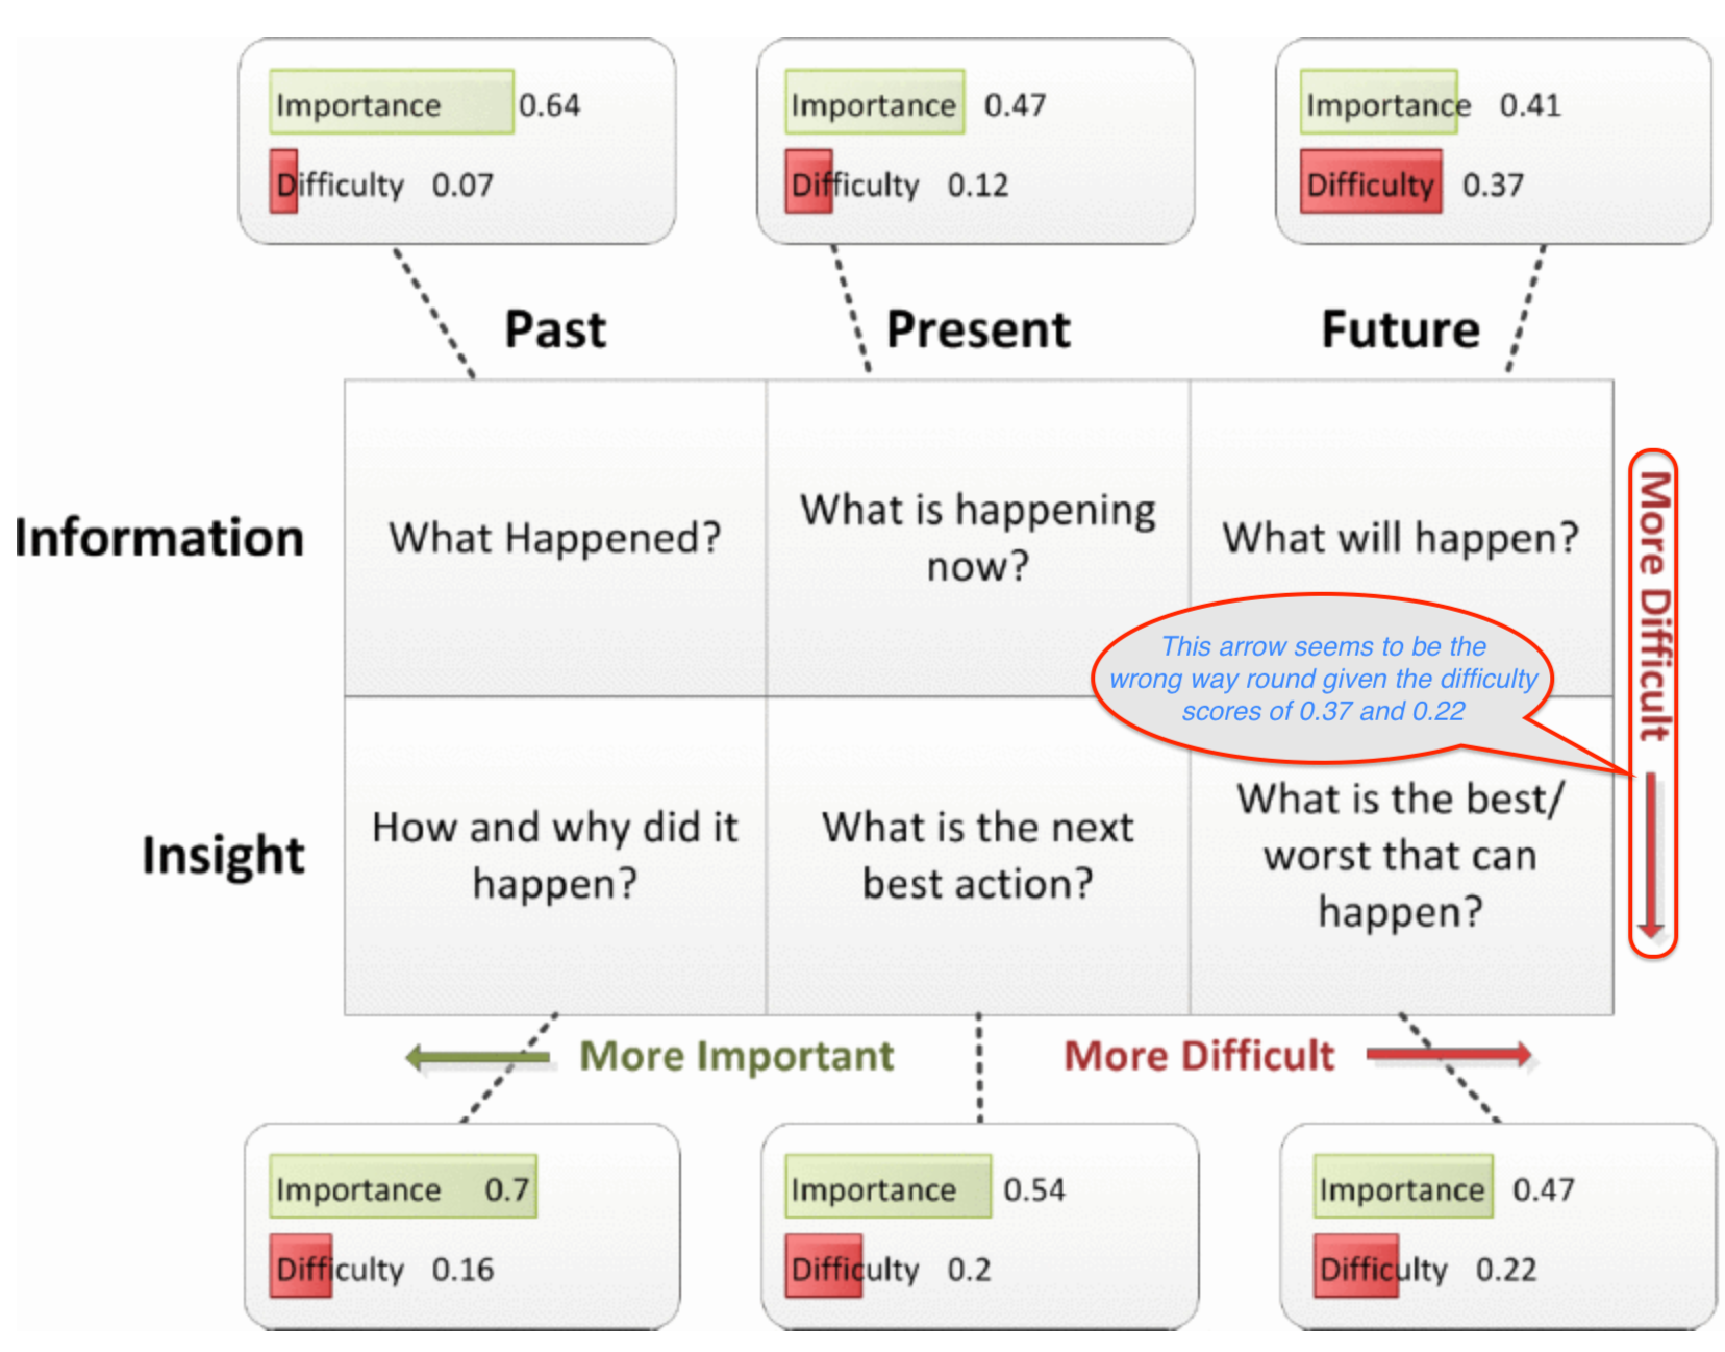
\includegraphics[width=\linewidth]{images/related-work/buse2012-edited-figure-2.pdf}
    \caption[Analytical questions, adapted from \cite{buse2012_information_needs_for_software_development_analytics}]{Revised Figure 2 from \cite{buse2012_information_needs_for_software_development_analytics}}
    \label{fig:buse2012-edited-figure-2}
\end{figure*}

Oddly, Figure 2 in their paper seems to have a mistake in the direction of More Difficult from Information to Insight, see~\ref{fig:buse2012-edited-figure-2}.